\documentclass[11pt]{article}

\usepackage[utf8]{inputenc}
\usepackage[T1]{fontenc}
\usepackage{kpfonts}
\usepackage{geometry}
\geometry{a4paper}

\usepackage{array}
\usepackage{amsmath}
\usepackage{longtable}
\usepackage{wrapfig}

\usepackage[frenchb,english]{babel}
\usepackage{graphicx}
%\usepackage{hyperref}

%%% PACKAGES
\usepackage{verbatim}
\usepackage{subfigure}
\usepackage{url}

%%% ToC (table of contents) APPEARANCE
\usepackage[nottoc,notlof,notlot]{tocbibind} % Put the bibliography in the ToC 

\title{Short manual for \TeX works}
\author{Alain Delmotte}
%\date{}

\begin{document}
\maketitle
\tableofcontents

\section{Introduction}

\TeX works is a project to create a text editor oriented for \LaTeX. Instead to create a new sophisticated editor, fully equipped by multiple tool-bars to meet any need, \TeX works on the contrary try to provide a simple editor, offering at first sight only some limited tools for text editing as well as one button and a menu to typeset a \LaTeX text.

The idea to create the editor came to Jonathan Kew, the initiator in charge of the project, after a long reflection on the reasons why potential users tend to keep away from \LaTeX, as well as from the success of the \TeX shop editor on the Mac.

Finally the goal was also to provide the same editor on many operating systems; \TeX works runs for the moment on Linux, Mac OS as well as Windows. The interface is always the same and the program offers the same possibilities.

The first section explain how to install the software. In the second one describes the interface and one creates a first document. In the third section one sees the advanced tools proposed by \TeX works; one should read this section only after mastering the basic working system of \TeX works. The tools presented allow to be much more effective. Finally the last section, as annexes, provides lists for the keyboard short-cuts, the commands known as regular expression, as well as the roots for auto-completion. A bibliography closes this introduction.

\section{Installation}
\label{insta}

\TeX works is only a text editor; to be able to create documents with \LaTeX{} and to typeset them to PDF, we need what is called a \TeX{} distribution. It is a bunch of programmes and other necessary files which will be automatically called by \TeX works during its work. So one needs to install a distribution; we will do that ``before'' to start \TeX works for the first time, this way \TeX works will automatically find what it needs.

One can use \textbf{TeXlive} (\url{http://www.tug.org/texlive/)} which is a combination of teTeX, macTeX and XEmTeX and which is available for the three operating systems. The last available version is TeXlive 2008.

For Linux: every Linux distribution has a \LaTeX{} distribution; but it could not be installed by default and one has to use the installation tools to do that. Except TeXlive, one can use \textbf{teTeX} (\url{http://www.tug.org/teTeX/} on which TeXlive is based.

For the mac: \textbf{MacTeX}, new distribution based on gwTeX and XeTeX. See also on the WEB at \url{http://www.tug.org/mactex/}.

For Windows: an often used distribution is \textbf{MiKTeX} (\url{http://www.miktex.org/}). MiKTeX has an update programme, which has also been ported to Linux. One can also use the XEmTeX distribution (\url{http://www.xemtex.org/}).

For \TeX works, download the archived programmes from the \TeX works web site: \url{htp://tug.org/texworks/}; one can find binaries for Mac and Windows at: \url{http://code.google.com/p/texworks/downloads/list}.

One has to get: \verb|TeXworksW32-r238.zip| (or \verb|TeXworksOSX-r238.zip| for the Mac), the programme itself, as well as \verb|TeXworksW32-libs-20080714.zip| (and for the Mac \verb|TeXworksOSX-libs-20080714.zip|), some needed library files \footnote{available versions at the time of writing this manual.}.

\subsection{Under Windows}

We create a folder, for example \verb+C:\Program files\TeXworks+, and un-archive the downloaded files in it. Create, on the desktop or in the quick launch bar a short-cut for the \verb+TeXworks.exe+ file.

When you start the program the first time, it creates in the folder associated to your account (\verb+C:\Documents and Settings\<vourname>\+) a folder named \verb+TeXworks+ which will contain some folders for the auto-completion, configuration, dictionaries, templates, and localisation files -- but we will see later. \footnote{\TeX works will save its preferences in the register:
\url{\HKEY_CURRENT_USER\Software\TUG\TeXworks}. If they are erased, they will be recreated with default values at the next use.}

NB. Up to the version used here, the fact that the name of the main folder of the user, in ``Documents and Settings'', has accented characters, in fact any non-ASCII character, will prevent the use of the spell-checker and of the automatic shift from the source to the view and back with positionning at the same place.

\subsection{Under Linux}

Under Linux, most of the time one build the programme by compiling; see the annexe at section \ref{compil}. Once the compilation is done, start \TeX works.

A folder \verb=.texworks= will be created in your \verb=home= directory.

\subsection{Under Mac OS}

Put the libraries and frameworks in the indicated folders, unless you already have them installed. 

On Mac OS X, the \TeX works resources folder will be created in your \verb=Library= folder, inside your \verb=home= directory. Preferences are stored in \url{ ~/Library/Preferences/org.tug.TeXworks.plist}
which you can delete if you ever suspect it is causing problems.

\section{First approach}

Let's now see how to do a first document: for this one has to type it in the editor window of \TeX works. \LaTeX{} is not a WYSIWIG software \footnote{\emph{What You See Is What You Get}}, so you'll have to type the text and the instructions for formatting it and you'll see the result only after ``typesetting'' the text.

This looks a little bit dry, but one very quickly gets used to it and this is worth the result.

\subsection{Short description of the interface}

When one opens the editor, it shows a very skinny(?) interface: a title bar, a menu bar, two small tool-bars, a great typing zone and, at the bottom, a status bar.
\vspace{10pt}

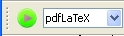
\includegraphics[scale=.6]{barreun}\hspace{10pt}%
The first tool-bar has a button to typeset and an unfolding menu to choose the format for typesetting (we'll choose \verb=pdfLaTeX=). Knowing that the keyboard short-cut for typesetting is \verb=CTRL+T= and that we almost never change the format, one could even not show this tool-bar. Further the selection can be done through the \textbf{Composition} menu.
\vspace{10pt}

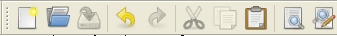
\includegraphics[scale=.6]{barredeux}\hspace{10pt}%
The second only provides classical buttons: New document, Open, Save | Undo, Redo | Cut, Copy, Paste | Search, Replace.

\subsection{Creating un document}

\subsubsection{Writing the document}

Let's create now the first document! Enter exactly the following text! \footnote{It is intentionally in French to show some possibilities!}

\noindent\rule{100mm}{0.5pt}
\begin{verbatim}
\documentclass{article}

\usepackage[utf8]{inputenc}
\usepackage[T1]{fontenc}
\usepackage{geometry}
\geometry{a4paper}

\usepackage[francais]{babel}

\title{Premier document}
\author{Un TeXnicien}
\date{}

\begin{document}
\maketitle

Voici un texte accentué en français!

\end{document}
\end{verbatim}
\noindent\rule{100mm}{0.5pt}

One have to save the document, putting it in a folder, which we specially create for the tests; the name of the document file, for example \verb=first.tex=, should have a \verb=.tex= extension.

\subsubsection{Typesetting the document and viewing it}

Next we start typesetting \footnote{We also use the words compilation and compile for the same action, indeed \LaTeX{} works on the source file to produce a .pdf output, so there is a compilation.} by clicking the green button \raisebox{-4pt}{
\includegraphics[scale=.4]{compo}} or by \verb=CTR+T=.

A new panel opens between the typing area and the status bar, it is the \emph{output panel}; there goes everything \LaTeX{} is doing when it works; when it is finished and if there is no error, this panel disappears and a new window appears next to the first one; in this window one can see a page with a title ``Premier document'' followed by the name of the author ``Un TeXnicien'', both centred, a text \foreignlanguage{frenchb}{``Voici un texte accentué en français!''} and at the bottom centre a page number.

Remark that the mouse cursor is like a magnifier! If you push the left button of the mouse you can see the text under the magnifier much bigger (it is a magnifier, isn't); you can move the magnifier and so inspect the text in details.

To go back to the source, you can just click in its window or better, you'll see by using, do \verb=CTRL+'=. This last short-cut is a toggle between the two windows. \footnote{Under Windows one can use \texttt{Alt+Tab} to go to the last window opened before the one in use.}

See also \ref{psourvue} the automatic move at a specified location of the view from the source or the inverse.

\subsubsection{The work of \LaTeX}

Let's now shortly analyse the result to understand what \LaTeX{} did and why. Introductions and full tutorials can be found on Internet; see for example \textit{lshort} which should be in the installed \LaTeX{} distribution or which can be downloaded from the net: do a search on CTAN. \footnote{\textit{Comprehensive TeX Archives Network}, it is a network of mirror deposits of the central CTAN, one can find there everything about \TeX{} and \LaTeX \url{http://www.ctan.org}}
%
%\noindent\raisebox{5pt}{\rule{50mm}{1pt}}
\vspace{5pt}

We ask to create a document of the class: \emph{article}, it is the global layout of the document.

Next we say that the input document (the source) is saved with the Unicode format utf-8 and that it will then contain characters which are not present in the standard ASCII without accents. We also want to use an output format T1; we also want an \emph{A4} document and not the us \emph{letter} format. Finally we make it clear that the typography should follow the French rules. Those general instructions for the work are done by packages called with options.

Lastly we finish the declaration part of the document, the preamble, giving the title, the author and the date of the document.

Next comes the body of the document, between \verb+\begin{document}+ and \verb+\end{document}+. It is here where everything which will appear in the document will be.

Let's do some experiments to show the effect of these instructions. For this we put an \% in front of the instructions; the \% and everything after it will be considered as comment, that part will then be ignored by \LaTeX. \footnote{Remark that the comments are coloured in red, so we see them well.}

Comment the lines loading the packages one after the other (\verb|\usepackage[]{}|). When you comment the French package, the typesetting will stop (for \LaTeX{} there is an error due to the previous work), just type \verb|[Enter]| to go on. Observe in details the result, for example with the magnifier the exclamation mark and the surrounding text; see also if all characters are present.

After these experiments, let's modify the text as follows:

\noindent\rule{100mm}{0.5pt}
\begin{verbatim}
\begin{document}
\maketitle
\tableofcontents

\section{Petite démonstration}

Voici un texte accentué en français!
Suite du texte entré après avoir fait un retour chariot. Dans l'éditeur 
on peut demander un passage à la ligne du texte saisi; mais le numéro de 
ligne n'est incrémenté que par un retour chariot.

Nouvelle ligne en passant une ligne dans la source: c'est la manière 
d'indiquer un changement de paragraphe.

\end{document}
\end{verbatim}
\noindent\rule{100mm}{0.5pt}

Redo the previous experiments and observe the changes which appear.

Note that entering only one carriage return doesn't create a new paragraph. In \LaTeX{} one has to have an empty line for that. In \TeX works the line number of the source (on the right in the status bar) numbers the lines created with carriage return, not the wrapped lines.

\subsection{And when errors occur}

When you create a document for typesetting with \LaTeX, you can avoid making mistakes: forgetting a closing brace or a \verb|\end{}| command to close an environment, no command to switch to the mathematical mode but use of mathematical commands,\dots{} When you compile, when there is an error, \LaTeX{} stops, this stop is visible by the stop of the scrolling actions in the output panel, an error message is displayed and \LaTeX{} waits an instruction to know what it should do: one sees the \emph{typing cursor} in the line between the output panel and the status bar.

Note that we can stop the typesetting, the green button changed to a red one with a white cross \raisebox{-4pt}{
\includegraphics[scale=.4]{stop}}, by clicking on that button or else with \verb|[CTR+T]|. The output panel is still visible and so one can still see the error message.

The error message is on many lines, like this:

\noindent\rule{100mm}{0.5pt}
\begin{verbatim}
! Undefined control sequence.
l.168 ... fermante ou d'une commande \veb
                                         +\end{}+ de fermeture d'un...

? 
\end{verbatim}
\noindent\rule{100mm}{0.5pt}

\LaTeX{} says that it doesn't recognize the command name, sometimes suggests to see the manual or to type \verb|h| (plus \verb|[Return]|) for help, points to the line number (here 168) and the place of the error at the cut of the line (here at \verb|\veb|) and finally with the question mark shows that it waits for an action from us.

There are different possible actions:
\begin{itemize}
\item type \verb+[Return]+ and ask to continue as if nothing happened; sometimes this allows to finish compiling, but there will be an error in the result;
\item type \verb+h[Return]+ to ask for help; this help in not always clearer than the error message, but often this gives a clue;
\item type \verb+i[Return]+ to tell \LaTeX{} that we will propose a replacement text, enter it followed by \verb|[Return]|, it will be used, beginning at the level of the error, but you should correct the source afterwards; there is no correction in the source during compilation;
\item type \verb=x[Return]= to stop compilation.
\end{itemize}

One should note that sometimes an error appears far from its real position, for example opening an environment but not closing it, \LaTeX{} doesn't see the error before it encounters another end of environment without closing of the first one; it is often the \verb|\end{document}| which shows that another environment was not closed!

\subsection{Changing a little bit \TeX works parameters for convenience}

If the default font of the editor doesn't suit you, it is possible to change it by \textsl{\textbf{Format / Font...}} and selection in the dialogue box which appears. This change will only be temporary, one gets back the default font if one closes \TeX works and opens it again.

From the \textsl{\textbf{Typeset}} menu or from the unfolding menu of the \textsl{\textbf{Typesetting tool bar}} one can change the compilation format. Again this change will only be temporary.

To have a permanent change, one has to change the \emph{preferences} through the \textsl{\textbf{Edition / Preferences...}} menu, panel \textsl{\textbf{Editor}} for the font and panel \textsl{\textbf{Typesetting}}, at the bottom, for the default format (let's choose \texttt{pdflatex} for this one).

\section{Going further with \TeX works}

When you'll have some practise with \TeX works, you'll find the need for more effective tools. Many tools exist in \TeX works. We are going to see them now.

\subsection{Spell-check}

One can ask to have automatic spell-check during typing by \textsl{\textbf{Edit / Spelling / <selection of the language>}}: as an example fr-FR for French.

During typing, if there is an error, the word is underlined by a red underline. A right-click on the word opens a contextual menu in which there are some replacement suggestions. Click on the desired word to make the replacement.

Before to use the spell-check, one has to install dictionaries in the right folder of \TeX works: \verb|C:\Documents and Settings\<yourname>\TeXworks\dictionaries|.

One can use the available dictionaries for Open office and other free software \footnote{see for example at \url{http://lingucomponent.openoffice.org/download_dictionary.html}}; for example, if you have Thunderbird with spell-check, you can copy the \verb|.aff| and \verb|.dic| files. it is possible to ask \TeX works to use by default a dictionary by \textsl{\textbf{Edit / Preferences\dots / Editor}} option \textsl{\textbf{Spell-check language:}}.

\subsection{Toggle source/view}

When one reads the document in the view and one sees an error, it is interesting to go immediately at the same place in the source. To do that it is enough to click at the selected place in the view holding \verb|[Ctrl]| down (\verb|[Ctrl+Click]|, one jumps to the searched location in the source.

De same way, if one has already shown the view and one is back in the source, one can go back to the view at a specific location by \verb|[Ctrl+Click]|.

\subsection{Creating a document from a template}

The documents that we create use most of the time the same instructions in the preamble, one loads the same packages, one specifies the same page layouts, one also specifies personal headers and footers,\dots

One can use predefined templates or create one's own having all those pre-requi\-re\-ments.

Use \textsl{\textbf{File / New from template...}} or \verb|Ctrl+Shift+N|. A dialogue box opens to allow selection of the template. After selection and \verb|OK| a document is created and one can start to work.

If one desires to create a more personal template, one has just to create this document with everything one always wants to find (and perhaps marking places to fill in) and save it as a \verb|.tex| files in the \TeX works folder or a possible sub-folder of this one \verb|C:\Documents and Settings\<yourname>\TeXworks\templates| \footnote{case of Windows, see section \ref{insta} Installation.}.

\subsection{Creating a project using several source files}

When the source becomes long, it is sometimes difficult to move in it. It is then interesting to split the source in different smaller files: one file will be the main document, central, with the preamble, the \verb|document| environment, as well as calls to the ``sub-documents'' \footnote{calls by the commands
\texttt{$\backslash$input\{\}} or \texttt{$\backslash$input\{\}}, see \LaTeX{} manuals for more information.}.

But there might be a problem if, being in a sub-document, on start typesetting/compilation; as there is no preamble nor \verb|document| environment there is an immediate error stop.

To tell \TeX works that it should typeset the main document one adds at the very beginning of the sub-document the instruction:

\verb|% !TeX root = chemin/au/fichier_principal.tex|

\noindent for example:

\verb|% !TeX root = manual.tex|

if the main file is in the same folder, its name is enough, as in the above example. Also remark the use of the slash ``\verb|/|'' and not the backslash ``\verb|\|'' used under Windows to separate the levels of folders.

\subsection{Other special commands}

The same way one can manage two other aspects of the compilation. \TeX works uses, by default, the ``utf8'' encoding, but some files could be saved in another format. To ask another encoding for a specific file one can put at the beginning of this file:

\verb|% !TeX encoding = latin1| : another encoding often used.

If one wants to compile a file by another programme than the default \TeX{} or \LaTeX{}, put at the beginning of the file:

\verb|% !TeX program = the_programme|.

\subsection{Classical editing tools and other}

\TeX works has the classical editing tools as the clipboard; therefore one can select, cut/copy and paste a piece of text.

One can select with the mouse by ``glide??'' on the desired text, one can also ``double-click'' to select a word. With the keyboard one moves holding the \verb|[Shift]| key down; one can use only the direction keys with \verb|[Shift]|; one can also move and select word by word moving left or right holding \verb|[Ctrl+Shift]| down. The clipboard short-cuts are the short-cuts one finds in all the programmes: \verb|[Ctrl-X]| to cut, \verb|[Ctrl+C]| to copy and \verb|[Ctrl+V]| to paste.

One can easily change the case of a selection -- put everything upper case or everything lower case -- by  \textsl{\textbf{Edit / Changer case /}} and next depending on the case \textsl{\textbf{ALL UPPER CASE}} or \textsl{\textbf{all lower case}}.

it is always possible to undo an un-wished action by \textsl{\textbf{Edit / Undo}} or \verb|[Ctrl+Z]|; this way one can undo stepwise! The inverse action undo the undo or redo is done by \textsl{\textbf{Edit / Redo}} or \verb|[Ctrl+Maj+Z]|.

When one prepare a document with \LaTeX{} it is often interesting to prevent compilation of a portion of text to be able to locate an error; one goes on this way piece by piece of good text until one finds a part which creates an error. For this one comments the source. 

We have seen that the symbol \texttt{\%} shows the beginning of a comment. To comment a big piece of text, it is enough to select it and ask to mark it as comment \textsl{\textbf{Format / Comment}} or \verb|Ctrl+Shift+]|. To suppress the comment: \textsl{\textbf{Format / Uncomment}} or \verb|Ctrl+Shift+[|. 

A frequent error is to forget a closing symbol: parenthesis, bracket, square bracket. \TeX works helps with a tool to show the pairs of symbols: when one move over one of these symbols its complementary is briefly highlighted in orange. One can also, when one is inside a block like this, one can ask to select the block by \textsl{\textbf{Edit / balance delimiters}} or by its short-cut \verb|[Ctrl+B]|. Thus one immediately sees the scope of the block.

\subsection{Search and replace}

other classical tools: search and replace text. Of course \TeX works has these possibilities with some more possibilities.

\subsubsection{Classical actions}

The options of the menu \textsl{\textbf{Search}}: ``\textsl{\textbf{Find\dots}}'', ``\textsl{\textbf{Find again}}'', ``\textsl{\textbf{Replace\dots}}'' et \textsl{\textbf{Replace again}} (\verb|[Ctrl+F|], \verb|[Ctrl+G]|, \verb|[Ctrl+R]| et \verb|[Ctrl+Shift+R]| respectively) are classical actions; the first and the third open a dialogue box:

\begin{center}
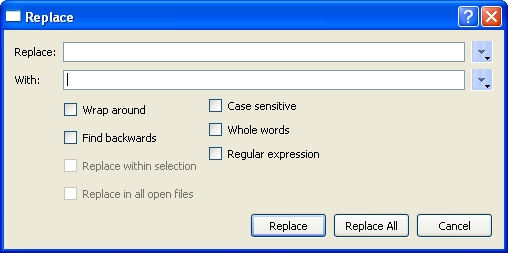
\includegraphics[scale=.6]{findrepl}
\end{center}

There are the usual options: \emph{search forwards} (default), \emph{Find backwards}, \emph{Wrap around} or \emph{Replace within selection}. The following options are also usual \emph{Case sensitive} and \emph{Whole words}.

The option \emph{Replace in all open files} is also a frequent extension, but not as much as the others; this allows, for example, to replace in all the files of a project.

The last option, \emph{Regular expression}, is detailed below.

In the menu \textsl{\textbf{Search}} there are other interesting options:
\begin{itemize}
\item \textsl{\textbf{Copy to Find}}, when one wants to search or replace some text by another one can select the text and send it in the input area \emph{Replace:} of the Replace dialogue box; for only searching without replacement one can also use this option, one then sends to the \emph{Find:} area of the Find dialogue box, but the third option described below is more practical in this case;
\item \textsl{\textbf{Copy to Replace}}, one does the same for the replacement text; it is then enough to launch Replace\dots{} (\verb|[Ctrl+R]|) and the information are already in the right areas;
\item \textsl{\textbf{Find Selection}}, with this it is even not necessary to send to the \emph{Find:} area, next open the dialog box by \verb|[Ctrl+F]|, it is enough to use the (\verb|[Ctrl+H]| command and \TeX works searches the next occurrence of the selection; one can repeat the search by \verb|[Ctrl+G]|;
\item \textsl{\textbf{Show selection}}, if one selects some text and after this ones moves somewhere else with mouse lateral slider, entering the \verb|[Ctrl+=]| brings us back to the selected text.
\end{itemize}

\subsubsection{Regular expressions}

The regular expressions provide a very powerful tool, but one has to understand them well. There are often used when one writes programmes, as well as in the programmes them-self to manage the content worked upon by the latests. A full manual would be required only to learn them, but we'll give some ideas on how to use. See also the available expressions in section \ref{regexp}.

Suppose we have the following text:
\begin{verbatim}
Voici du texte pour tester les expressions régulières 
dans du texte accentué. 
Voici du texte pour tester les expressions régulières dans 
du texte accentué. 
Voici du texte pour tester les expressions régulières. Voici 
du texte pour tester les expressions régulières. 
truc          truc
tél.: 010-99-99-99
tél.: 00.32.10.99.99.99
tél.: 00/32-10/99.99.99
\end{verbatim}
We want to 1) insert an empty line between the paragraphs after ``accentué'' (paragraph in \LaTeX) but not for the three telephone numbers, we also want 2) replace the two tabulations between the two words ``truc'' of the fourth paragraph, each by three spaces and finally 3) make uniform the telephone numbers replacing the ``\verb+-./+'' by spaces. 

For 1) in the dialogue box \textsl{\textbf{Replace}} (\verb![Ctrl+R]!) for \emph{Find:} we put ``\verb+>\n<+'' \footnote{here the \texttt{><} only show the limits of the typed text and should not be typed them-self.} and in \emph{With:} ``\verb+>\n\n<+''. ``\verb+\n+'' is the code to insert a line feed. One would take care to first select the first four paragraphs and the beginning of the fifth (first telephone number) and to mark off the \emph{Replace within selection}; if this is not done, select the telephone lines and do the reverse action ``\verb+>\n\n<+'' and ``\verb+>\n<+''.

For 2) use ``\verb+>\t<+'' and ``\verb*+>   <+''. ``\verb+\t+'' is the code which represent a tabulation.

For 3) it will be ``\verb+>-|\.|/<+'' and ``\verb*+> <+''. Here ``\verb+|+'' provides different possibilities; for the point we have used ``\verb+\.+'' because the dot alone represents any character and we would have replaced all the characters by a space!! we then use a code to get the point.

If on has strings of the same character but of different length (for example 2, 3, 4, 5 characters) and one wants to bring all strings to a string with less characters (for example 2), one can ask to replace the string ``\verb+>e{3,5}<+'' by ``\verb+>ee<+''.

If one wants to insert at the beginning of some paragraphs separated or not by an empty line the same string, for example \verb*+\noindent + or \verb*+\item +, one can replace ``\verb+>\n\n<+'' or ``\verb+>\n<+'' by ``\verb*+>\n\n\\noindent <+'' or ``\verb*+>\n\\noindent <+''. pay attention, we have double \verb|\| in front of \verb|noindent|!

If it was making sense, we could replace all the letters between ``a'' and ``m'' by ``\$'' using ``\verb+>[a-m]<+'' and ``\verb+>$<+''.

\subsection{Auto-completion}

Another tool which rapidly becomes indispensable is auto-completion. Indeed, when one uses \LaTeX, ones has continuously to enter codes for, for example, create environments; further in this case one has to remember to close them.

The auto-completion allows to type a string, one could say a keyword, and next typing \verb|[Tab]| the \LaTeX{} command or environment code is automatically created.

As an example to have ``\LaTeX'', we have to type \verb|\LaTeX|. This is not difficult, but entering ``\verb|\|'' \footnote{in particular on some keyboard, like the French Azerty one, to have $\backslash$ it is necessary to use \texttt{[AltGr+<]} or \texttt{[Ctrl+Alt+<]}} followed by the word ``\verb|LaTeX|'' with alternating capitals and lower case letters could become annoying after a while. With auto-completion you just enter  \verb|latex| next \verb|[TaB]| to get \verb|\LaTeX|. One just have to take care that there is no \emph{letter} glued in front or after \verb|latex|.

Other examples, \verb|bmin| gives:
\begin{verbatim}
\begin{minipage}{}
•
\end{minipage}
\end{verbatim}
the blinking insert location is between the empty pair of brackets where one has to enter the size of the minipage, and \verb|xve| gives \verb|\varepsilon| that is $\varepsilon$ in mathematical mode. See the section \ref{autoc} for a list of the keywords for auto-completion. Remark the ``•'' in the minipage environment. It is  a place holder which can be reached by \verb|[Option+Tab]| on the Mac, repeating this one goes forward in the created structure and by \verb|[Maj+Option+Tab]| one goes backward. \footnote{ This doesn't work yet with Windows, under Linux ??}

One should remark that if a partial keyword is given and that uses repeatedly \verb|[Tab]|, one can have other completions, generally associated. For example, \verb|bali| (the \verb|b| means the beginning of an environment \verb|\begin{}|) creates the \verb|align| environment after one \verb|[Tab]|, next \verb|align*|, and after, in succession, \verb|alignat|, \verb|alignat*|, \verb|aligned|, \verb|alignedat|, \verb|alignedat| with option; these last environments have their own code which starts by \verb|bali| (\verb|balis baliat baliats balied baliedat| and \verb|baliedato|.)

Eventually, if you want to create your own short-cuts/keywords, you can add a \verb|.txt| file in the \verb|completion| of the \verb|TeXworks| folder created during the first use (see section \ref{dostexw} on installation.) 

The entries in the file should have the following format:
\begin{verbatim}
bfigo:=\begin{figure}[#INS#]#RET##RET#\end{figure}
\bibliography{#INS#}
\end{verbatim}

In the first case, for the \verb|figure| environment with option, \verb|bfigo| is the keyword, next comes the assignment \verb|:=| and the definition: write \verb|\begin{figure}[] \end{figure}| with a line feed after \verb|begin| (\verb|#RET#|), create an empty line (second \verb|#RET#|) and put the cursor between the square brackets (\verb|#INS#|).

In the second case there will be only \verb|\bibliography{}| it-self and the cursor between the brackets. The keyword is the instruction itself.

Of course it is always possible to use ``•''!

One has to take care to create utf-8 encoded files; they can be created with \TeX works it-self.

\subsection{Formatting the source for legibility}

To facilitate legibility of the source, one can use the indentation as the programmers are doing:
\begin{verbatim}
\begin{itemize}
    \item First element of the list;
    \item second element;
    \item last element:
    \begin{itemize}      % beginning of the sub-list
        \item first sub-element;
        \item second sub-element.
    \end{itemize}
\end{itemize}
\end{verbatim}
this increases legibility, but works well only on short lines, without text wrapping; or if one ask not to use text wrapping by \textsl{\textbf{Format / Wrap lines}}.

The command \textsl{\textbf{Format / Indent}} or the short-cut \verb|Ctrl+]| will indent the line, or the selected lines, moving four characters. One can repeat the process to increase the indent. Each time there is insertion of a tabulation character in the source.

To suppress one indentation: \textsl{\textbf{Format / Unindent}} or the short-cut \verb|Ctrl+[|.

\subsection{Showing the tags}

When a document is becoming long and one wants to move to a specific place (a chapter, a section, a sub-section,\dots) one has to scroll the edition window to find the desired location.

One can also ask to show the structure tags of the document in a panel to the left of the edition panel by \textsl{\textbf{Window / Show / Balises}}; the same instruction allows to mask this panel, as well as a click on the cross in the upper right corner of the panel. A click on the searched level selects the corresponding instruction of the source.

One can even more or less develop the structure if it is very long by a click on the small square with ``-'' to reduce/close a structure and on the small square with ``+'' to open it.

The same action is possible in the view by \textsl{\textbf{Window / Show / Table of contents}}, but this only works if one has created structure tags  in the PDF file using the package \verb|hyperref|.

\subsection{Organising the windows}

By default, the edition window opens on the left and the view one, when the corresponding PDF file exists, to the right splitting the screen in two.

One can change the position of the windows in the menu \textsl{\textbf{Window}}. \textsl{\textbf{Stack}} and \textsl{\textbf{Side by side}} give the same effect if there is only one document open, if not Stack creates a mosaic with all the windows. The other options allow to place the windows for one's convenience. It is also always possible to re-size and move the windows.

For the view one can change the way it is presented and of course the zoom by \textsl{\textbf{Actual size}}, \textsl{\textbf{Fit to width}} and \textsl{\textbf{Fit to window}} using the options of the \textsl{\textbf{View}} menu; one can also zoom in and out. Short-cuts exist for all these actions and are given next to the option in the menu.
\newpage

\section{Annexes}
\subsection{Keyboard short-cuts}

The use of keyboard short-cuts greatly facilitate typing in and the management of the source and the preview. Their use is much more effective than the use of the mouse on tool-bars' buttons.

You'll find here below the short-cuts for the work in the source and those for the preview

\newcolumntype{P}{>{\ttfamily}p{20mm}}

For the work in the source:

\begin{longtable}{Pp{60mm}}
\textrm{Short-cut} & Action\\
\hline Ctrl+N & New\\
Ctrl+Maj+N & New from template\\
Ctrl+O & Open\\
Ctrl+S & Save\\
Ctrl+Maj+S & Save as\\
Ctrl+W & Close\\
Ctrl+Z & Undo\\
Ctrl+Maj+Z & Redo\\
Ctrl+X & Cut\\
Ctrl+C & Copy\\
Ctrl+V & Paste\\
Ctrl+F & Search\\
Ctrl+G & Search again\\
Ctrl+R & Replace\\
Ctrl+E & Copy to Find\\
Ctrl+Maj+E & Copy to replace\\
Ctrl+L & Go to line\\
Ctrl+H & Find selection\\
Ctrl+= & Show selection\\
Ctrl+A & Select All\\
Ctrl+B & Balance Delimiters\\
Ctrl+] & Indent\\
Ctrl+[ & Unindent\\
Ctrl+Maj+] & Comment\\
Ctrl+Maj+[ & Uncomment\\
Ctrl+\ & Show/hide output panel\\
Ctrl+' & Go to preview\\
Tab & Auto-completion\\
\\
\multicolumn{2}{l}{moves (and selections: \texttt{Shift+})}\\
$\rightarrow$ & 1 character right\\
Ctrl+$\rightarrow$ & 1 word right\\
$\leftarrow$ & 1 character left\\
Ctrl+$\leftarrow$ & 1 word left\\
$\uparrow$ & 1 line up\\
$\downarrow$ & 1 line down\\
PgUp & 1 screen up\\
PgDown & 1 screen down\\
Home & Begin of line\\
Ctrl+Home & Begin of document\\
End & End of line\\
Ctrl+End & End of document\\
\end{longtable}

For the work in preview:

\begin{longtable}{Pp{60mm}}
\textrm{Short-cut} & Action\\
\hline Ctrl+N & New\\
Ctrl+Maj+N & New from template\\
Ctrl+O & Open\\
Ctrl+W & Close\\
Ctrl+Z & Undo\\
Ctrl+Maj+Z & Redo\\
Ctrl+X & Cut\\
Ctrl+C & Copy\\
Ctrl+V & Paste\\
Ctrl+RetArr & Erase\\
Home & First page\\
End & Last page\\
PgUp & Previous page\\
PgDown & Next page\\
Ctrl+G & Go to page\dots\\
Ctrl++ & Zoom +\\
Ctrl+- & Zoom -\\
Ctrl+1 & Actual size\\
Ctrl+2 & Fit to width\\
Ctrl+3 & Fit to window\\
Ctrl+Maj+F & Full screen\\
Ctrl+T & Typeset\\
Ctrl+' & Go to source\\
\end{longtable}



\subsection{Regular expressions}
\label{regexp}

================================> to be written

\subsection{Roots for completion}
\label{autoc}

We give here the keywords for auto-completion as they are supplied by \TeX works. They are in the files \verb|tw-basic.txt|, \verb|tw-context.txt| (empty) and \verb|tw-latex.txt| from the \verb|TeXworks\Completion| folder.

We give them in three columns: the first two show the keywords, the third the \LaTeX{} code produced. In some cases therre is only the code, this means that one can starts to enter the \LaTeX{} code and try to complete  it by \verb|[Tab]|.

During completion, the system inserts line feeds and puts the cursor at the first place where one has to enter information to complete the typing. To represent the line feeds we used $\mathcal{R}$ and $\mathcal{I}$ for the input point.

It is possible to see that the keywords have some coherence, the mathematical variables have a keyword starting with \verb|x|, when they are in a mathematical environment, when they are used alone in the text one adds \verb|d| in front; for example \verb|xa| and \verb|dxa| for \verb|\alpha|, if there is a capital there is a \verb|c|, as  \verb|xo| for \verb|\omega| and \verb|xco| for \verb|\Omega|. The keywords for environments start with \verb|b|: \verb|bali| for
\verb|align| (\verb|b| for \verb|\begin|). When the environment has possible options, there is one or more \verb|o| added to the base name: \verb|bminp| for \verb|\begin{minipage}{}..| and 
\verb|bminpo| for \verb|\begin{minipage}[]{}..|.
\vspace{12pt}

Keywords defined in \verb|tw-basic.txt| (defined in \TeX):
\ttfamily
\begin{longtable}{p{20mm}p{20mm}p{65mm}}
xa & $\backslash$xa & $\backslash$alpha\\
xb & $\backslash$xb & $\backslash$beta\\
xch & $\backslash$xch & $\backslash$chi\\
xd & $\backslash$xd & $\backslash$delta\\
xcd & $\backslash$xcd & $\backslash$Delta\\
xe & $\backslash$xe & $\backslash$epsilon\\
xve & $\backslash$xve & $\backslash$varepsilon\\
xet & $\backslash$xet & $\backslash$eta\\
xg & $\backslash$xg & $\backslash$gamma\\
xcg & $\backslash$xcg & $\backslash$Gamma\\
xio & $\backslash$xio & $\backslash$iota\\
xl & $\backslash$xl & $\backslash$lambda\\
xcl & $\backslash$xcl & $\backslash$Lambda\\
xm & $\backslash$xm & $\backslash$mu\\
xn & $\backslash$xn & $\backslash$nu\\
xo & $\backslash$xo & $\backslash$omega\\
xco & $\backslash$xco & $\backslash$Omega\\
xp & $\backslash$xp & $\backslash$pi\\
xcp & $\backslash$xcp & $\backslash$Pi\\
xvp & $\backslash$xvp & $\backslash$varpi\\
xph & $\backslash$xph & $\backslash$phi\\
xcph & $\backslash$xcph & $\backslash$Phi\\
xvph & $\backslash$xvph & $\backslash$varphi\\
xps & $\backslash$xps & $\backslash$psi\\
xcps & $\backslash$xcps & $\backslash$Psi\\
xs & $\backslash$xs & $\backslash$sigma\\
xcs & $\backslash$xcs & $\backslash$Sigma\\
xvs & $\backslash$xvs & $\backslash$varsigma\\
xz & $\backslash$xz & $\backslash$zeta\\
xr & $\backslash$xr & $\backslash$rho\\
xvr & $\backslash$xvr & $\backslash$varrho\\
xt & $\backslash$xt & $\backslash$tau\\
xth & $\backslash$xth & $\backslash$theta\\
xcth & $\backslash$xcth & $\backslash$Theta\\
xvth & $\backslash$xvth & $\backslash$vartheta\\
xu & $\backslash$xu & $\backslash$upsilon\\
xcu & $\backslash$xcu & $\backslash$Upsilon\\
xx & $\backslash$xx & $\backslash$xi\\
xcx & $\backslash$xcx & $\backslash$Xi\\
tex & $\backslash$tex & $\backslash$TeX\\
 &  & $\backslash$TeX\\
texs & $\backslash$texs & $\backslash$TeX$\backslash$ \\
 &  & $\backslash$TeX$\backslash$ \\
 & $\backslash$bsk & $\backslash$bigskip\\
 &  & $\backslash$bigskip$\mathcal{R}$\\
 &  & $\backslash$hskip\\
 &  & $\backslash$indent\\
 &  & $\backslash$input\\
 & $\backslash$msk & $\backslash$medskip\\
 &  & $\backslash$medskip$\mathcal{R}$\\
 &  & $\backslash$noindent\\
 &  & $\backslash$par\\
 & $\backslash$ssk & $\backslash$smallskip$\mathcal{R}$\\
 &  & $\backslash$smallskip$\mathcal{R}$\\
 &  & $\backslash$scriptsize\\
 &  & $\backslash$vskip\\
\end{longtable}
\rmfamily

Keywords defined in \verb|tw-latex.txt|:
\ttfamily
\begin{longtable}{p{20mm}p{20mm}p{65mm}}
-- &  & $\backslash$textendash\\
-- &  & $\backslash$textendash$\backslash$ \\
--- &  & $\backslash$textemdash\\
--- &  & $\backslash$textemdash$\backslash$ \\
 &  & $\backslash$author\{$\mathcal{I}$\}$\mathcal{R}$\\
 &  & $\backslash$begin\{\\
adlen & $\backslash$adl & $\backslash$addtolength\{$\mathcal{I}$\}\{\}$\mathcal{R}$\\
 &  & $\backslash$addtolength\{$\mathcal{I}$\}\{\}\\
adcount & $\backslash$adc & $\backslash$addtocounter\{$\mathcal{I}$\}\{\}$\mathcal{R}$\\
 &  & $\backslash$addtocounter\{$\mathcal{I}$\}\{\}\\
barr &  & $\backslash$begin\{array\}$\mathcal{RIR}\backslash$end\{array\}\\
babs & $\backslash$babs & $\backslash$begin\{abstract\}$\mathcal{RIR}\backslash$end\{abstract\}\\
bali & $\backslash$bali & $\backslash$begin\{align\}$\mathcal{RIR}\backslash$end\{align\}\\
balis & $\backslash$balis & $\backslash$begin\{align*\}$\mathcal{RIR}\backslash$end\{align*\}\\
baliat & $\backslash$baliat & $\backslash$begin\{alignat\}\{$\mathcal{I}$\}$\mathcal{RR}\backslash$end\{alignat\}\\
baliats & $\backslash$baliats & $\backslash$begin\{alignat*\}\{$\mathcal{I}$\}$\mathcal{RR}\backslash$end\{alignat*\}\\
balied & $\backslash$balied & $\backslash$begin\{aligned\}\{$\mathcal{I}$\}$\mathcal{RR}\backslash$end\{aligned\}\\
baliedat & $\backslash$baliedat & $\backslash$begin\{alignedat\}$\mathcal{RIR}\backslash$end\{alignedat\}\\
baliedato & $\backslash$baliedato & $\backslash$begin\{alignedat\}[$\mathcal{I}$]$\mathcal{RR}\backslash$end\{alignedat\}\\
bapp & $\backslash$bapp & $\backslash$begin\{appendix\}$\mathcal{RIR}\backslash$end\{appendix\}\\
bbmat & $\backslash$bbmat & $\backslash$begin\{bmatrix\}$\mathcal{RIR}\backslash$end\{bmatrix\}\\
bcase & $\backslash$bcase & $\backslash$begin\{cases\}$\mathcal{RIR}\backslash$end\{cases\}\\
bcent & $\backslash$bcent & $\backslash$begin\{center\}$\mathcal{RIR}\backslash$end\{center\}\\
bcenum & $\backslash$bcenum & $\backslash$begin\{compactenum\}$\mathcal{R}\backslash$item$\mathcal{RIR}\backslash$end\{compactenum\}\\
bcenumo & $\backslash$bcenumo & $\backslash$begin\{compactenum\}[$\mathcal{I}$]R$\backslash$item$\mathcal{RR}\backslash$end\{compactenum\}\\
bcitem & $\backslash$bcitem & $\backslash$begin\{compactitem\}$\mathcal{R}\backslash$item$\mathcal{RIR}\backslash$end\{compactitem\}\\
bcitemo & $\backslash$bcitemo & $\backslash$begin\{compactitem\}[$\mathcal{I}$]R$\backslash$item$\mathcal{RR}\backslash$end\{compactitem\}\\
bdes & $\backslash$bdes & $\backslash$begin\{description\}$\mathcal{R}\backslash$item[$\mathcal{I}$]$\mathcal{RR}\backslash$end\{description\}\\
benu & $\backslash$benu & $\backslash$begin\{enumerate\}$\mathcal{R}\backslash$item$\mathcal{RIR}\backslash$end\{enumerate\}\\
benuo & $\backslash$benuo & $\backslash$begin\{enumerate\}[$\mathcal{I}$]R$\backslash$item$\mathcal{RR}\backslash$end\{enumerate\}\\
bequ & $\backslash$bequ & $\backslash$begin\{equation\}$\mathcal{RIR}\backslash$end\{equation\}\\
bequs & $\backslash$bequs & $\backslash$begin\{equation*\}$\mathcal{RIR}\backslash$end\{equation*\}\\
beqn & $\backslash$beqn & $\backslash$begin\{eqnarray\}$\mathcal{RIR}\backslash$end\{eqnarray\}\\
beqns & $\backslash$beqns & $\backslash$begin\{eqnarray*\}$\mathcal{RIR}\backslash$end\{eqnarray*\}\\
bf & $\backslash$bf & $\backslash$textbf\{$\mathcal{I}$\}\\
bfd & $\backslash$bfseries & $\backslash$bfseries\\
bfig & $\backslash$bfig & $\backslash$begin\{figure\}$\mathcal{RIR}\backslash$end\{figure\}\\
bfigo & $\backslash$bfigo & $\backslash$begin\{figure\}[$\mathcal{I}$]$\mathcal{RR}\backslash$end\{figure\}\\
bmult &  & $\backslash$begin\{multiline\}$\mathcal{RIR}\backslash$end\{multiline\}\\
bflalig & $\backslash$bflalig & $\backslash$begin\{flalign\}$\mathcal{RIR}\backslash$end\{flalign\}\\
bflaligs & $\backslash$bflaligs & $\backslash$begin\{flalign*\}$\mathcal{RIR}\backslash$end\{flalign*\}\\
bfll & $\backslash$bfll & $\backslash$begin\{flushleft\}$\mathcal{RIR}\backslash$end\{flushleft\}\\
bflr & $\backslash$bflr & $\backslash$begin\{flushright\}$\mathcal{RIR}\backslash$end\{flushright\}\\
bgath & $\backslash$bgath & $\backslash$begin\{gather\}$\mathcal{RIR}\backslash$end\{gather\}\\
bgaths & $\backslash$bgaths & $\backslash$begin\{gather*\}$\mathcal{RIR}\backslash$end\{gather*\}\\
bgathed & $\backslash$bgathed & $\backslash$begin\{gathered\}$\mathcal{RIR}\backslash$end\{gathered\}\\
bgathedo & $\backslash$bgathedo & $\backslash$begin\{gathered\}[$\mathcal{I}$]$\mathcal{RR}\backslash$end\{gathered\}\\
bite & $\backslash$bite & $\backslash$begin\{itemize\}$\mathcal{R}\backslash$item$\mathcal{RIR}\backslash$end\{itemize\}\\
biteo & $\backslash$biteo & $\backslash$begin\{itemize\}[$\mathcal{I}$]R$\backslash$item$\mathcal{RR}\backslash$end\{itemize\}\\
biblio &  & $\backslash$bibliography\{$\mathcal{I}$\}\\
bibstyle & $\backslash$bibstyle & $\backslash$bibliographystyle\{$\mathcal{I}$\}\\
blett & $\backslash$blett & $\backslash$begin\{letter\}\{$\mathcal{I}$\}$\mathcal{RR}\backslash$end\{letter\}\\
blist & $\backslash$blist & $\backslash$begin\{list\}\{$\mathcal{I}$\}\{\}$\mathcal{R}\backslash$item$\mathcal{RR}\backslash$end\{list\}\\
bminp & $\backslash$bminp & $\backslash$begin\{minipage\}\{$\mathcal{I}$\}$\mathcal{RR}\backslash$end\{minipage\}\\
bminpo & $\backslash$bminpo & $\backslash$begin\{minipage\}[$\mathcal{I}$]\{\}$\mathcal{RR}\backslash$end\{minipage\}\\
bmult & $\backslash$bmult & $\backslash$begin\{multiline\}$\mathcal{RIR}\backslash$end\{multiline\}\\
bmults & $\backslash$bmults & $\backslash$begin\{multiline*\}$\mathcal{RIR}\backslash$end\{multiline*\}\\
botr &  & $\backslash$bottomrule$\mathcal{R}$\\
bpict & $\backslash$bpict & $\backslash$begin\{picture\}$\mathcal{RIR}\backslash$end\{picture\}\\
bpmat & $\backslash$bpmat & $\backslash$begin\{pmatrix\}$\mathcal{RIR}\backslash$end\{pmatrix\}\\
bquot & $\backslash$bquot & $\backslash$begin\{quotation\}$\mathcal{RIR}\backslash$end\{quotation\}\\
bquo & $\backslash$bquo & $\backslash$begin\{quote\}$\mathcal{RIR}\backslash$end\{quote\}\\
bsplit & $\backslash$bsplit & $\backslash$begin\{split\}$\mathcal{RIR}\backslash$end\{split\}\\
bsubeq & $\backslash$bsubeq & $\backslash$begin\{subequations\}$\mathcal{RIR}\backslash$end\{subequations\}\\
btab & $\backslash$btab & $\backslash$begin\{tabular\}\{$\mathcal{I}$\}$\mathcal{RR}\backslash$end\{tabular\}\\
btabs & $\backslash$btabs & $\backslash$begin\{tabular*\}\{$\mathcal{I}$\}\{\}$\mathcal{RR}\backslash$end\{tabular*\}\\
btabx & $\backslash$btabx & $\backslash$begin\{tabularx\}\{$\mathcal{I}$\}\{\}$\mathcal{RR}\backslash$end\{tabularx\}\\
btabl & $\backslash$btabl & $\backslash$begin\{table\}$\mathcal{RIR}\backslash$end\{table\}\\
btablo & $\backslash$btablo & $\backslash$begin\{table\}[$\mathcal{I}$]$\mathcal{RR}\backslash$end\{table\}\\
btabls & $\backslash$btabls & $\backslash$begin\{table*\}$\mathcal{RIR}\backslash$end\{table*\}\\
btablso & $\backslash$btablso & $\backslash$begin\{table*\}[$\mathcal{I}$]$\mathcal{RR}\backslash$end\{table*\}\\
btbl & $\backslash$btbl & $\backslash$begin\{table\}$\mathcal{RIR}\backslash$end\{table\}\\
btblo & $\backslash$btblo & $\backslash$begin\{table\}[$\mathcal{I}$]$\mathcal{RR}\backslash$end\{table\}\\
btbls & $\backslash$btbls & $\backslash$begin\{table*\}$\mathcal{RIR}\backslash$end\{table*\}\\
btblso & $\backslash$btblso & $\backslash$begin\{table*\}[$\mathcal{I}$]$\mathcal{RR}\backslash$end\{table*\}\\
btabb & $\backslash$btabb & $\backslash$begin\{tabbing\}$\mathcal{RIR}\backslash$end\{tabbing\}\\
bbib & $\backslash$bbib & $\backslash$begin\{thebibliography\}\{$\mathcal{I}$\}$\mathcal{R}\backslash$bibitem\{\} $\mathcal{RR}\backslash$end\{thebibliography\}\\
bindex & $\backslash$bindex & $\backslash$begin\{theindex\}$\mathcal{RIR}\backslash$end\{theindex\}\\
btheo & $\backslash$btheo & $\backslash$begin\{theorem\}$\mathcal{RIR}\backslash$end\{theorem\}\\
btitpg & $\backslash$btitpg & $\backslash$begin\{titlepage\}$\mathcal{RIR}\backslash$end\{titlepage\}\\
btrivl & $\backslash$btrivl & $\backslash$begin\{trivlist\}$\mathcal{RIR}\backslash$end\{trivlist\}\\
bvarw & $\backslash$bvarw & $\backslash$begin\{varwidth\}\{$\mathcal{I}$\}$\mathcal{RR}\backslash$end\{varwidth\}\\
bverb & $\backslash$bverb & $\backslash$begin\{verbatim\}$\mathcal{RIR}\backslash$end\{verbatim\}\\
bvers & $\backslash$bvers & $\backslash$begin\{verse\}$\mathcal{RIR}\backslash$end\{verse\}\\
bibitem &  & $\backslash$bibitem\{$\mathcal{I}$\}$\mathcal{R}$\\
bibitemo &  & $\backslash$bibitem[$\mathcal{I}$]\{\}$\mathcal{R}$\\
 &  & $\backslash$bottomrule$\mathcal{R}$\\
 &  & $\backslash$boxed\{$\mathcal{I}$\}\\
center &  & $\backslash$centering\\
chap & $\backslash$chapter\{$\mathcal{I}$\} & $\backslash$chapter\{$\mathcal{I}$\}$\mathcal{R}$\\
 &  & $\backslash$cite\{$\mathcal{I}$\}\\
 &  & $\backslash$citep\{$\mathcal{I}$\}\\
 &  & $\backslash$citet\{$\mathcal{I}$\}\\
 &  & $\backslash$caption\{$\mathcal{I}$\}$\mathcal{R}$\\
 &  & $\backslash$cdots\\
 &  & $\backslash$cline\{$\mathcal{I}$\}\\
cmidr &  & $\backslash$cmidrule(I)\{\}\\
cmidro &  & $\backslash$cmidrule[$\mathcal{I}$]()\{\}\\
 &  & $\backslash$date\{$\mathcal{I}$\}$\mathcal{R}$\\
dd & $\backslash$dd & $\backslash$($\mathcal{I}\backslash$)\\
 &  & $\backslash$ddots\\
 &  & $\backslash$ddot\{$\mathcal{I}$\}\\
 &  & $\backslash$dddot\{$\mathcal{I}$\}\\
 &  & $\backslash$ddddot\{$\mathcal{I}$\}\\
 &  & $\backslash$documentclass\{$\mathcal{I}$\}$\mathcal{R}$\\
 &  & $\backslash$documentclass[$\mathcal{I}$]\{\}$\mathcal{R}$\\
 &  & $\backslash$dots\\
 &  & $\backslash$dotsc\\
 &  & $\backslash$dotsb\\
 &  & $\backslash$dotsm\\
 &  & $\backslash$dotsi\\
 &  & $\backslash$dotso\\
em & $\backslash$emph\{$\mathcal{I}$\} & $\backslash$emph\{$\mathcal{I}$\}\\
emd &  & $\backslash$em\\
 &  & $\backslash$end\{$\mathcal{I}$\}$\mathcal{R}$\\
 &  & $\backslash$eqref\{$\mathcal{I}$\}\\
foot & $\backslash$footnote\{$\mathcal{I}$\} & $\backslash$footnote\{$\mathcal{I}$\}\\
 &  & $\backslash$footnotesize\\
fbox &  & $\backslash$fbox\{$\mathcal{I}$\}\\
fboxo & $\backslash$fboxo & $\backslash$framebox[$\mathcal{I}$]\{\}\\
 &  & $\backslash$framebox[$\mathcal{I}$]\{\}\\
fboxoo & $\backslash$fboxoo & $\backslash$framebox[$\mathcal{I}$][]\{\}\\
 &  & $\backslash$framebox[$\mathcal{I}$][]\{\}\\
 &  & $\backslash$fboxrule\{$\mathcal{I}$\}\\
 &  & $\backslash$fboxsep\{$\mathcal{I}$\}\\
geometry & $\backslash$geometry\{\} & $\backslash$geometry\{\}\\
 &  & $\backslash$hline$\mathcal{R}$\\
 &  & $\backslash$hspace\{$\mathcal{I}$\}\\
 &  & $\backslash$hspace*\{$\mathcal{I}$\}\\
hw &  & $\backslash$headwidth\\
hw2tw &  & $\backslash$setlength\{$\backslash$headwidth\}\{$\backslash$textwidth\}$\mathcal{R}$\\
href &  & $\backslash$href\{$\mathcal{I}$\}\{\}\\
 &  & $\backslash$include\{$\mathcal{I}$\}$\mathcal{R}$\\
incg &  & $\backslash$includegraphics\{$\mathcal{I}$\}$\mathcal{R}$\\
incgo &  & $\backslash$includegraphics[$\mathcal{I}$]\{\}$\mathcal{R}$\\
it &  & $\backslash$item$\mathcal{RI}$\\
ito &  & $\backslash$item[$\mathcal{I}$]$\mathcal{R}$\\
 &  & $\backslash$intertext\{$\mathcal{I}$\}\\
ti & $\backslash$ti & $\backslash$textit\{$\mathcal{I}$\}\\
itd & $\backslash$itshape & $\backslash$itshape\\
latex & $\backslash$latex & $\backslash$LaTeX\\
 &  & $\backslash$LaTeX\\
latexs & $\backslash$latexs & $\backslash$LaTeX$\backslash$ \\
 &  & $\backslash$LaTeX$\backslash$ \\
latexe & $\backslash$latexe & $\backslash$LaTeXe\\
 &  & $\backslash$LaTeXe\\
latexes & $\backslash$latexes & $\backslash$LaTeXe$\backslash$ \\
 &  & $\backslash$LaTeXe$\backslash$ \\
lbl & $\backslash$lbl & $\backslash$label\{$\mathcal{I}$\}\\
 &  & $\backslash$label\{$\mathcal{I}$\}\\
 &  & $\backslash$large\\
 &  & $\backslash$Large\\
 &  & $\backslash$ldots\\
listf & $\backslash$listf & $\backslash$listoffigures$\mathcal{R}$\\
 &  & $\backslash$listoffigures$\mathcal{R}$\\
listt & $\backslash$listt & $\backslash$listoftables$\mathcal{R}$\\
 &  & $\backslash$listoftables$\mathcal{R}$\\
mbf & $\backslash$mbf & $\backslash$mathbf\{$\mathcal{I}$\}\\
 &  & $\backslash$mathbf\{$\mathcal{I}$\}\\
mrm & $\backslash$mrm & $\backslash$mathrm\{$\mathcal{I}$\}\\
 &  & $\backslash$mathrm\{$\mathcal{I}$\}\\
mcal & $\backslash$mcal & $\backslash$mathcal\{$\mathcal{I}$\}\\
 &  & $\backslash$mathcal\{$\mathcal{I}$\}\\
msf & $\backslash$msf & $\backslash$mathsf\{$\mathcal{I}$\}\\
 &  & $\backslash$mathsf\{$\mathcal{I}$\}\\
mtt & $\backslash$mtt & $\backslash$mathtt\{$\mathcal{I}$\}\\
 &  & $\backslash$mathtt\{$\mathcal{I}$\}\\
mit & $\backslash$mit & $\backslash$mathit\{$\mathcal{I}$\}\\
 &  & $\backslash$mathit\{$\mathcal{I}$\}\\
mnorm & $\backslash$mnorm & $\backslash$mathnormal\{$\mathcal{I}$\}\\
 &  & $\backslash$mathnormal\{$\mathcal{I}$\}\\
mdd &  & $\backslash$mdseries\\
mbox &  & $\backslash$mbox\{$\mathcal{I}$\}\\
 &  & \\
mboxo & $\backslash$mboxo & $\backslash$makebox[$\mathcal{I}$]\{\}\\
 &  & $\backslash$makebox[$\mathcal{I}$]\{\}\\
mboxoo & $\backslash$mboxoo & $\backslash$makebox[$\mathcal{I}$][]\{\}\\
 &  & $\backslash$makebox[$\mathcal{I}$][]\{\}\\
mpar & $\backslash$mpar & $\backslash$marginpar\{$\mathcal{I}$\}\\
 &  & $\backslash$marginpar\{$\mathcal{I}$\}\\
midr &  & $\backslash$midrule$\mathcal{R}$\\
multc & $\backslash$multc & $\backslash$multicolumn\{$\mathcal{I}$\}\{\}\{\}\\
multic & $\backslash$multic & $\backslash$multicolumn\{$\mathcal{I}$\}\{\}\{\}\\
 &  & $\backslash$multicolumn\{$\mathcal{I}$\}\{\}\{\}\\
ncol & $\backslash$ncol &  \& \\
ncm &  & $\backslash$newcommand\{$\mathcal{I}$\}\{\}$\mathcal{R}$\\
newc &  & $\backslash$newcommand\{$\mathcal{I}$\}\{\}$\mathcal{R}$\\
ncmo &  & $\backslash$newcommand\{$\mathcal{I}$\}[]\{\}$\mathcal{R}$\\
newco &  & $\backslash$newcommand\{$\mathcal{I}$\}[]\{\}$\mathcal{R}$\\
ncmoo &  & $\backslash$newcommand\{$\mathcal{I}$\}[][]\{\}$\mathcal{R}$\\
newcoo &  & $\backslash$newcommand\{$\mathcal{I}$\}[][]\{\}$\mathcal{R}$\\
nct &  & $\backslash$newcolumntype\{$\mathcal{I}$\}\{\}\\
newct &  & $\backslash$newcolumntype\{$\mathcal{I}$\}\{\}\\
newpg &  & $\backslash$newpage$\mathcal{R}$\\
npg & $\backslash$npg & $\backslash$newpage$\mathcal{R}$\\
nline &  & $\backslash$newline$\mathcal{R}$\\
newlin &  & $\backslash$newline$\mathcal{R}$\\
nlen &  & $\backslash$newlength\{$\mathcal{I}$\}$\mathcal{R}$\\
newlen &  & $\backslash$newlength\{$\mathcal{I}$\}$\mathcal{R}$\\
nenv &  & $\backslash$newenvironment\{$\mathcal{I}$\}\{\}\{\}$\mathcal{R}$\\
newe &  & $\backslash$newenvironment\{$\mathcal{I}$\}\{\}\{\}$\mathcal{R}$\\
nenvo &  & $\backslash$newenvironment\{$\mathcal{I}$\}[]\{\}\{\}$\mathcal{R}$\\
neweo &  & $\backslash$newenvironment\{$\mathcal{I}$\}[]\{\}\{\}$\mathcal{R}$\\
nenvoo &  & $\backslash$newenvironment\{$\mathcal{I}$\}[][]\{\}\{\}$\mathcal{R}$\\
neweoo &  & $\backslash$newenvironment\{$\mathcal{I}$\}[][]\{\}\{\}$\mathcal{R}$\\
newt &  & $\backslash$newtheorem\{$\mathcal{I}$\}\{\}$\mathcal{R}$\\
newto &  & $\backslash$newtheorem\{$\mathcal{I}$\}\{\}[]$\mathcal{R}$\\
newtoo &  & $\backslash$newtheorem\{$\mathcal{I}$\}[]\{\}$\mathcal{R}$\\
 &  & $\backslash$nocite\{$\mathcal{I}$\}\\
 &  & $\backslash$normalsize\\
pgref &  & $\backslash$pageref\{$\mathcal{I}$\}\\
par &  & $\backslash$paragraph\{$\mathcal{I}$\}$\mathcal{R}$\\
pars &  & $\backslash$paragraph*\{$\mathcal{I}$\}$\mathcal{R}$\\
paro &  & $\backslash$paragraph[$\mathcal{I}$]\{\}$\mathcal{R}$\\
 &  & $\backslash$pagebreak$\mathcal{R}$\\
pgs &  & $\backslash$pagestyle\{$\mathcal{I}$\}$\mathcal{R}$\\
parbox &  & $\backslash$parbox\{$\mathcal{I}$\}\{\}\\
parboxo &  & $\backslash$parbox[$\mathcal{I}$]\{\}\{\}\\
pbox & $\backslash$pbox & $\backslash$parbox\{$\mathcal{I}$\}\{\}\\
pboxo & $\backslash$pboxo & $\backslash$parbox[$\mathcal{I}$]\{\}\{\}\\
pbox &  & $\backslash$pbox\{$\mathcal{I}$\}\{\}\\
ref &  & $\backslash$ref\{$\mathcal{I}$\}\\
rncm &  & $\backslash$renewcommand\{$\mathcal{I}$\}\{\}$\mathcal{R}$\\
rnewc &  & $\backslash$renewcommand\{$\mathcal{I}$\}\{\}$\mathcal{R}$\\
rnewco &  & $\backslash$renewcommand\{$\mathcal{I}$\}[]\{\}$\mathcal{R}$\\
rncmo &  & $\backslash$renewcommand\{$\mathcal{I}$\}[]\{\}$\mathcal{R}$\\
rnewcoo &  & $\backslash$renewcommand\{$\mathcal{I}$\}[][]\{\}$\mathcal{R}$\\
rncmoo &  & $\backslash$renewcommand\{$\mathcal{I}$\}[][]\{\}$\mathcal{R}$\\
 &  & $\backslash$rm\\
rmc &  & $\backslash$rmfamily\\
rbox & $\backslash$rbox & $\backslash$raisebox\{$\mathcal{I}$\}\{\}\\
 &  & $\backslash$raisebox\{$\mathcal{I}$\}\{\}\\
rboxo & $\backslash$rboxo & $\backslash$raisebox\{$\mathcal{I}$\}[]\{\}\\
 &  & $\backslash$raisebox\{$\mathcal{I}$\}[]\{\}\\
rboxoo & $\backslash$rboxoo & $\backslash$raisebox\{$\mathcal{I}$\}[][]\{\}\\
 &  & $\backslash$raisebox\{$\mathcal{I}$\}[][]\{\}\\
 &  & $\backslash$rule\{$\mathcal{I}$\}\{\}\\
 &  & $\backslash$rule[$\mathcal{I}$]\{\}\{\}\\
 &  & $\backslash$sc\\
 &  & $\backslash$scshape\\
sec &  & $\backslash$section\{$\mathcal{I}$\}$\mathcal{R}$\\
secs &  & $\backslash$section*\{$\mathcal{I}$\}$\mathcal{R}$\\
seco &  & $\backslash$section[$\mathcal{I}$]\{\}$\mathcal{R}$\\
 &  & $\backslash$setlength\{$\mathcal{I}$\}\{\}\\
ssec & $\backslash$ssec & $\backslash$subsection\{$\mathcal{I}$\}$\mathcal{R}$\\
 &  & $\backslash$subsection\{$\mathcal{I}$\}$\mathcal{R}$\\
ssecs & $\backslash$ssecs & $\backslash$subsection*\{$\mathcal{I}$\}$\mathcal{R}$\\
 &  & $\backslash$subsection*\{$\mathcal{I}$\}$\mathcal{R}$\\
sseco & $\backslash$sseco & $\backslash$subsection[$\mathcal{I}$]\{\}$\mathcal{R}$\\
 &  & $\backslash$subsection[$\mathcal{I}$]\{\}$\mathcal{R}$\\
sssec & $\backslash$sssec & $\backslash$subsubsection\{$\mathcal{I}$\}$\mathcal{R}$\\
 &  & $\backslash$subsubsection\{$\mathcal{I}$\}$\mathcal{R}$\\
sssecs & $\backslash$sssecs & $\backslash$subsubsection*\{$\mathcal{I}$\}$\mathcal{R}$\\
 &  & $\backslash$subsubsection*\{$\mathcal{I}$\}$\mathcal{R}$\\
ssseco & $\backslash$ssseco & $\backslash$subsubsection[$\mathcal{I}$]\{\}$\mathcal{R}$\\
 &  & $\backslash$subsubsection[$\mathcal{I}$][]$\mathcal{R}$\\
spar & $\backslash$spar & $\backslash$subparagraph\{$\mathcal{I}$\}\\
 &  & $\backslash$subparagraph\{$\mathcal{I}$\}\\
spars & $\backslash$spars & $\backslash$subparagraph*\{$\mathcal{I}$\}\\
 &  & $\backslash$subparagraph*\{$\mathcal{I}$\}\\
sparo & $\backslash$sparo & $\backslash$subparagraph[$\mathcal{I}$]\{\}\\
 &  & $\backslash$subparagraph[$\mathcal{I}$]\{\}\\
stcount &  & $\backslash$stepcounter\{$\mathcal{I}$\}$\mathcal{R}$\\
sf & $\backslash$sf & $\backslash$textsf\{$\mathcal{I}$\}\\
sfd & $\backslash$sffamily & $\backslash$sffamily\\
scd &  & $\backslash$scshape\\
sl & $\backslash$sl & $\backslash$textsl\{$\mathcal{I}$\}\\
 &  & $\backslash$textsl\{$\mathcal{I}$\}\\
sld &  & $\backslash$slshape\\
 &  & $\backslash$text\{$\mathcal{I}$\}\\
 &  & $\backslash$textbf\{$\mathcal{I}$\}\\
 &  & $\backslash$textsf\{$\mathcal{I}$\}\\
sc &  & $\backslash$textsc\{$\mathcal{I}$\}\\
 &  & $\backslash$textit\{$\mathcal{I}$\}\\
 &  & $\backslash$textup\{$\mathcal{I}$\}\\
tt & $\backslash$tt & $\backslash$texttt\{$\mathcal{I}$\}\\
ttd &  & $\backslash$ttfamily\\
 &  & $\backslash$texttt\{$\mathcal{I}$\}\\
tw & $\backslash$tw & $\backslash$textwidth\\
 &  & $\backslash$textwidth\\
 &  & $\backslash$thanks\{$\mathcal{I}$\}$\mathcal{R}$\\
 &  & $\backslash$title\{$\mathcal{I}$\}$\mathcal{R}$\\
tilde & $\backslash$tilde & $\backslash$textasciitilde\\
topr &  & $\backslash$toprule$\mathcal{R}$\\
toc & $\backslash$toc & $\backslash$tableofcontents$\mathcal{R}$\\
tableofcontents &  & $\backslash$tableofcontents$\mathcal{R}$\\
up & $\backslash$up & $\backslash$textup\{$\mathcal{I}$\}\\
upd &  & $\backslash$upshape\\
url &  & $\backslash$url\{$\mathcal{I}$\}\\
usep &  & $\backslash$usepackage\{$\mathcal{I}$\}$\mathcal{R}$\\
usepo &  & $\backslash$usepackage[$\mathcal{I}$]\{\}$\mathcal{R}$\\
 &  & $\backslash$vdots\\
 &  & $\backslash$vspace\{$\mathcal{I}$\}$\mathcal{R}$\\
 &  & $\backslash$vspace*\{$\mathcal{I}$\}$\mathcal{R}$\\
dxa & $\backslash$dxa & $\backslash$($\backslash$alpha$\backslash$)\\
dxb & $\backslash$dxb & $\backslash$($\backslash$beta$\backslash$)\\
dxch & $\backslash$dxch & $\backslash$($\backslash$chi$\backslash$)\\
dxd & $\backslash$dxd & $\backslash$($\backslash$delta$\backslash$)\\
dxcd & $\backslash$dxcd & $\backslash$($\backslash$Delta$\backslash$)\\
dxe & $\backslash$dxe & $\backslash$($\backslash$epsilon$\backslash$)\\
dxve & $\backslash$dxve & $\backslash$($\backslash$varepsilon$\backslash$)\\
dxet & $\backslash$dxet & $\backslash$($\backslash$eta$\backslash$)\\
dxg & $\backslash$dxg & $\backslash$($\backslash$gamma$\backslash$)\\
dxcg & $\backslash$dxcg & $\backslash$($\backslash$Gamma$\backslash$)\\
dxio & $\backslash$dxio & $\backslash$($\backslash$iota$\backslash$)\\
dxl & $\backslash$dxl & $\backslash$($\backslash$lambda$\backslash$)\\
dxcl & $\backslash$dxcl & $\backslash$($\backslash$Lambda$\backslash$)\\
dxm & $\backslash$dxm & $\backslash$($\backslash$mu$\backslash$)\\
dxn & $\backslash$dxn & $\backslash$($\backslash$nu$\backslash$)\\
dxo & $\backslash$dxo & $\backslash$($\backslash$omega$\backslash$)\\
dxco & $\backslash$dxco & $\backslash$($\backslash$Omega$\backslash$)\\
dxp & $\backslash$dxp & $\backslash$($\backslash$pi$\backslash$)\\
dxcp & $\backslash$dxcp & $\backslash$($\backslash$Pi$\backslash$)\\
dxvp & $\backslash$dxvp & $\backslash$($\backslash$varpi$\backslash$)\\
dxph & $\backslash$dxph & $\backslash$($\backslash$phi$\backslash$)\\
dxcph & $\backslash$dxcph & $\backslash$($\backslash$Phi$\backslash$)\\
dxvph & $\backslash$dxvph & $\backslash$($\backslash$varphi$\backslash$)\\
dxps & $\backslash$dxps & $\backslash$($\backslash$psi$\backslash$)\\
dxcps & $\backslash$dxcps & $\backslash$($\backslash$Psi$\backslash$)\\
dxs & $\backslash$dxs & $\backslash$($\backslash$sigma$\backslash$)\\
 & $\backslash$dxcs & $\backslash$($\backslash$Sigma$\backslash$)\\
dxvs & $\backslash$dxvs & $\backslash$($\backslash$varsigma$\backslash$)\\
dxz & $\backslash$dxz & $\backslash$($\backslash$zeta$\backslash$)\\
dxr & $\backslash$dxr & $\backslash$($\backslash$rho$\backslash$)\\
dxvr & $\backslash$dxvr & $\backslash$($\backslash$varrho$\backslash$)\\
dxt & $\backslash$dxt & $\backslash$($\backslash$tau$\backslash$)\\
dxth & $\backslash$dxth & $\backslash$($\backslash$theta$\backslash$)\\
dxcth & $\backslash$dxcth & $\backslash$($\backslash$Theta$\backslash$)\\
dxvth & $\backslash$dxvth & $\backslash$($\backslash$vartheta$\backslash$)\\
dxu & $\backslash$dxu & $\backslash$($\backslash$upsilon$\backslash$)\\
dxcu & $\backslash$dxcu & $\backslash$($\backslash$Upsilon$\backslash$)\\
dxx & $\backslash$dxx & $\backslash$($\backslash$xi$\backslash$)\\
dxcx & $\backslash$dxcx & $\backslash$($\backslash$Xi$\backslash$)\\
sqrt & $\backslash$sqrt & $\backslash$sqrt\{$\mathcal{I}$\}\\
sqrto & $\backslash$sqrto & $\backslash$sqrt[$\mathcal{I}$]\{\}\\
frac &  & $\backslash$frac\{$\mathcal{I}$\}\{\}\\
\end{longtable}
\rmfamily

\ttfamily
\begin{longtable}{p{100mm}}
\{array\}$\mathcal{RIR}\backslash$end\{array\}\\
\{abstract\}$\mathcal{RIR}\backslash$end\{abstract\}\\
\{align\}$\mathcal{RIR}\backslash$end\{align\}\\
\{align*\}$\mathcal{RIR}\backslash$end\{align*\}\\
\{alignat\}\{$\mathcal{I}$\}$\mathcal{RR}\backslash$end\{alignat\}\\
\{alignat*\}\{$\mathcal{I}$\}$\mathcal{RR}\backslash$end\{alignat*\}\\
\{aligned\}$\mathcal{RIR}\backslash$end\{aligned\}\\
\{aligned\}[$\mathcal{I}$]$\mathcal{RR}\backslash$end\{aligned\}\\
\{alignedat\}\{$\mathcal{I}$\}$\mathcal{RR}\backslash$end\{alignedat\}\\
\{appendix\}$\mathcal{RIR}\backslash$end\{appendix\}\\
\{bmatrix\}$\mathcal{RIR}\backslash$end\{bmatrix\}\\
\{compactenum\}$\mathcal{R}\backslash$item$\mathcal{RIR}\backslash$end\{compactenum\}\\
\{compactenum\}[$\mathcal{I}$]R$\backslash$item$\mathcal{RR}\backslash$end\{compactenum\}\\
\{compactitem\}$\mathcal{R}\backslash$item$\mathcal{RIR}\backslash$end\{compactitem\}\\
\{compactitem\}[$\mathcal{I}$]R$\backslash$item$\mathcal{RR}\backslash$end\{compactitem\}\\
\{cases\}$\mathcal{RIR}\backslash$end\{cases\}\\
\{center\}$\mathcal{RIR}\backslash$end\{center\}\\
\{description\}$\mathcal{R}\backslash$item[$\mathcal{I}$]$\mathcal{RR}\backslash$end\{description\}\\
\{enumerate\}$\mathcal{R}\backslash$item$\mathcal{RIR}\backslash$end\{enumerate\}\\
\{enumerate\}[$\mathcal{I}$]R$\backslash$item$\mathcal{RR}\backslash$end\{enumerate\}\\
\{equation\}$\mathcal{RIR}\backslash$end\{equation\}\\
\{eqnarray\}$\mathcal{RIR}\backslash$end\{eqnarray\}\\
\{eqnarray*\}$\mathcal{RIR}\backslash$end\{eqnarray*\}\\
\{figure\}$\mathcal{RIR}\backslash$end\{figure\}\\
\{figure\}[$\mathcal{I}$]$\mathcal{RR}\backslash$end\{figure\}\\
\{flalign\}$\mathcal{RIR}\backslash$end\{flalign\}\\
\{flalign*\}$\mathcal{RIR}\backslash$end\{flalign*\}\\
\{flushleft\}$\mathcal{RIR}\backslash$end\{flushleft\}\\
\{flushright\}$\mathcal{RIR}\backslash$end\{flushright\}\\
\{gather\}$\mathcal{RIR}\backslash$end\{gather\}\\
\{gather*\}$\mathcal{RIR}\backslash$end\{gather*\}\\
\{gathered\}$\mathcal{RIR}\backslash$end\{gathered\}\\
\{gathered\}[$\mathcal{I}$]$\mathcal{RR}\backslash$end\{gathered\}\\
\{itemize\}$\mathcal{R}\backslash$item$\mathcal{RIR}\backslash$end\{itemize\}\\
\{itemize\}[$\mathcal{I}$]R$\backslash$item$\mathcal{RR}\backslash$end\{itemize\}\\
\{letter\}\{$\mathcal{I}$\}$\mathcal{RR}\backslash$end\{letter\}\\
\{list\}\{$\mathcal{I}$\}\{\}$\mathcal{R}\backslash$item$\mathcal{RR}\backslash$end\{list\}\\
\{minipage\}\{$\mathcal{I}$\}$\mathcal{RR}\backslash$end\{minipage\}\\
\{minipage\}[$\mathcal{I}$]\{\}$\mathcal{RR}\backslash$end\{minipage\}\\
\{multiline\}$\mathcal{RIR}\backslash$end\{multiline\}\\
\{multiline*\}$\mathcal{RIR}\backslash$end\{multiline*\}\\
\{picture\}$\mathcal{RIR}\backslash$end\{picture\}\\
\{pmatrix\}$\mathcal{RIR}\backslash$end\{pmatrix\}\\
\{quotation\}$\mathcal{RIR}\backslash$end\{quotation\}\\
\{quote\}$\mathcal{RIR}\backslash$end\{quote\}\\
\{split\}$\mathcal{RIR}\backslash$end\{split\}\\
\{subequations\}$\mathcal{RIR}\backslash$end\{subequations\}\\
\{tabular\}\{$\mathcal{I}$\}$\mathcal{RR}\backslash$end\{tabular\}\\
\{tabular*\}\{$\mathcal{I}$\}\{\}$\mathcal{RR}\backslash$end\{tabular*\}\\
\{tabularx\}\{$\mathcal{I}$\}\{\}$\mathcal{RR}\backslash$end\{tabularx\}\\
\{table\}$\mathcal{RIR}\backslash$end\{table\}\\
\{table\}[$\mathcal{I}$]$\mathcal{RR}\backslash$end\{table\}\\
\{table*\}$\mathcal{RIR}\backslash$end\{table*\}\\
\{table*\}[$\mathcal{I}$]$\mathcal{RR}\backslash$end\{table*\}\\
\{tabbing\}$\mathcal{RIR}\backslash$end\{tabbing\}\\
\{thebibliography\}$\mathcal{RIR}\backslash$end\{thebibliography\}\\
\{theindex\}$\mathcal{RIR}\backslash$end\{theindex\}\\
\{theorem\}$\mathcal{RIR}\backslash$end\{theorem\}\\
\{titlepage\}$\mathcal{RIR}\backslash$end\{titlepage\}\\
\{trivlist\}$\mathcal{RIR}\backslash$end\{trivlist\}\\
\{varwidth\}\{$\mathcal{I}$\}$\mathcal{RR}\backslash$end\{varwidth\}\\
\{verbatim\}$\mathcal{RIR}\backslash$end\{verbatim\}\\
\{verse\}$\mathcal{RIR}\backslash$end\{verse\}\\
\end{longtable}
\rmfamily

There are also environment codes (above) without \verb|\begin{| (which is itself a keyword); this allows, if one started to input an environment code, to finish it by \verb|[Tab]|.

\subsection{Compiling \TeX works under Linux}
\label{compil}

From the \TeX works web site.

\textbf{Requirements}

To build the current TeXworks prototype from source, you will need to install developer packages (or equivalent) for: 

Qt4(4.3.2 is known to work; later versions should also work. Note that on GNU/ Linux, TeXworks may crash when changing the spell-checking language when using Qt~4.3.x. Updating to Qt 4.4.0 solves this.)

\noindent\url{http://trolltech.com/downloads/opensource#qt-open-source-edition}

Poppler (0.8.0 or later recommended, although 0.6 series should work) 

\noindent\url{http://poppler.freedesktop.org/}

Hunspell (at least 1.2.2 recommended; not tested with earlier versions) 

\noindent\url{http://hunspell.sourceforge.net/}

libdbus (on X11-based platforms only; not used on Mac OS X or Windows) 

\noindent\url{http://dbus.freedesktop.org/}

along with their dependencies (such as Freetype,fontconfig, zlib, etc.) 

Details will depend on your platform. 

On GNU/Linux or similar systems, your package manager can probably provide all these. Feel free to contribute distribution-specific notes for the Building page. 

After installing the necessary libraries (and their headers), check the TeXworks.pro file and update paths as necessary; some of the paths currently in the project file are specific to one of my build machines.

Once the project file is correct, run qmake to create a Makefile or Xcode project, and then run make or use Xcode to build the application. Do not run qmake -pro to recreate the .pro file, as it has been hand-edited. 

Note: on some systems, the default qmake may be a Qt3 version, in which case it will generate lots of warnings, and make will fail miserably; TeXworks is a Qt4 program. In that case, see if you have qmake-qt4, or perhaps run the Qt4 version using a full path. 

The current version of TeXworks has been successfully built with 
\begin{itemize}
\item Xcode (using gcc 4) on Mac OS X 10.4 and 10.5 
\item gcc 4 on GNU/Linux 
\item a combination of mingw32 on Windows XP and the mingw32 cross-compiler hosted on Mac OS X 
\end{itemize}

Getting all the right libraries built and installed for the mingw32 build can be tricky. By slightly patching poppler 0.8.0, it is possible to build a version that does not depend on fontconfig (and thence on various other libraries), though it will then not work properly for PDFs with non-embedded fonts. 

To avoid having to build the poppler dependencies for Windows, you can get precompiled libraries from the KDE on Windows project. 

Alternatively, I believe it would also be possible to build with Visual C, but I have not done this personally.  

\textbf{Notes on building TeXworks on various distributions.}

Building TeXworks on typical GNU/Linux systems should be fairly straightforward. You just need standard build tools (gcc, make, etc.), and the development files (not just runtime libraries) for Qt4, poppler,hunspell, and dbus. The exact set of packages needed will depend how your distribution arranges things; some examples are given here. 

\textsl{Fedora 9}
\begin{verbatim}
# yum install poppler-devel qt4-devel hunspell-devel
$ svn checkout http://texworks.googlecode.com/svn/trunk/ texworks-read-only
$ cd texworks-read-only
$ qmake
$ make
$ ./texworks
\end{verbatim}
(Thanks to Dave Crossland for this.) 

\textsl{Ubuntu (Hardy) \& Debian}
\begin{verbatim}
$ sudo aptitude install build-essential libpoppler-qt4-dev libhunspell-dev libdbus-1-dev
$ svn checkout http://texworks.googlecode.com/svn/trunk/ texworks-read-only
$ cd texworks-read-only
$ qmake-qt4
$ make
$ ./texworks
\end{verbatim}

(I hope this is OK; have not checked on a completely virgin Ubuntu system, so it is possible I missed something in the dependencies.) 

Another option would be to use the Ubuntu package announced by Martin Sievers, thus avoiding the need to compile from source.     
\newpage

\begin{thebibliography}{xx}
\bibitem{dkn1}\textbf{D. Knuth}, \textsl{The \TeX book}, Addison Wesley, 1986-1992

\bibitem{dkn2}\textbf{D. Knuth}, \textsl{The METAFONT book}, Addison Wesley, 1986-1992

\bibitem{lla}\textbf{L. Lamport}, \textsl{\LaTeX, user's guide and
reference manual}, Addison Wesley, 1985 (\LaTeX 2.09), 1994 (\LaTeX 2$\epsilon$)

\bibitem{gms}\textbf{M. Goossens, F. Mittelbach \& A. Samarin}, \textsl{The \LaTeX\ Companion}, Addison Wesley, 1994

\end{thebibliography}

\end{document}
